\chapter{Encoding FEC Chain} \label{chap:encoder}

% In this document explain all the things which I have done until the midterm presentation.
% All the details, Optimization techniques I have employed.
% Following text might be useful for writing the text.
% Also my midterm presentations/office presentations will be really useful for writing this part.  
% Reference paper for explaining the different components of the this FEC chain "Design of Polar codes for 5G NR radio"

%Work I have done Until now.
%
%%****************Optimizations to the original implementations until now.
%%****************Generic optimizations
%- Using optimization primitives such as likely and unlikely.
%- Aligning memory to 32 bytes so copying of data can be vectorized.
%- Polar transform optimization	
%- Replace binary additions with xor. instead of addition and then modulus two.
%- division and multiplications by left and right shift operations.
%- Avoided copy operations in polarTransform operations.
%****************Optimization in getting reliability indices.
%- Avoided remove and erase operations which have huge overhead. Wrote a efficient mechanism(reduced the latency by 176 us).
%- Instead removing and erasing I mark the element as removed.
%- Since the reliability indexes won't change. I built a look up table in place of searching all (1024)indices reduced the latency by 40us
%- Avoided copying operations of interleaved indexes.
%- Unrolled the loop to reduce the jumps.
%****************Rate matching optimizations.
%- optimization in subblock interleaving, Rewrote the logic to avoid E number of division and modulus operations.
%- Unrolled the for loops in subblock inteleaving method.
%- Implemented optimal version of bit selection, Avoided E number of modulus operations which are very costly.
%- Again optimization primitives for helping the branch predictor.
%
%
%Fast version of Encoding API's.
%In the original implementation of the polar encoding each of the bit is treated as 32 bit integer. This is highly inefficient
%when the goal is to process multiple bits at time. With each bit considered as 32 bit integer SIMD instructions won't provide
%any performance improvement. Reason is SIMD instruction can process multiple bits at time. avx2 instructions 256bits at a time.
%if we have 32 bits to represent a single bit. we can process only 8 bits at time. Which doesn't significantly improve the
%performance. To avoid this disadvantage and make use of SIMD capability. each 64 bit integer is considered as 64 bits of data.
%so one avx2 instruction can process 256 data bits in a single instruction.
%- Built a look up table to avoid last eight stages of polar encoding instead of traversing till end of tree.
%- Implemented SIMD instruction based encoding. Encoding happens within 0.6 us for N = 512.
%- Implemented optimal version of CRC calculation which can calculate CRC for PDCCH chain within 0.8 us. Original implementation was taking 7 us.
%- Implemented a bit interleaver which can deal with this format of data.

In this section, complete polar encoding FEC chain used in 5G is explained. Methods used for code profiling and latency measurement are presented. After figuring out the latency contributors code optimization/algorithm optimizations employed during the FEC chain development are presented and then presents how SIMD feature of the modern processors is exploited to obtain the low latency for PBCH and PDCCH FEC chains and frozen set selection algorithm improvement with the aid of look up table, finally presents the encoding process as traversal of a binary tree and how the encoding latency can be improved by pruning the tree hence avoiding the tree traversal instead using a lookup table to obtain the encoded result.

In 5G framework, Polar codes are used in downlink to encode downlink control information (DCI) over physical downlink control channel (PDCCH) and for payload in physical broadcast channel (PBCH). In uplink, to encode uplink control information (UCI) over the physical uplink control channel (PUCCH) and the physical uplink shared channel (PUSCH). In this work, notations introduced in 3GPP technical specification\cite{3gpp.38.212} are used.

The figure ~\ref{fig:5g_txfec_chain} represents the complete polar FEC chain for PBCH and PDCCH in downlink. Let's look at each of the components briefly to understand the FEC chain. In general $A$ bits have to be transmitted over a code of length $E$ code bits. $L$ CRC bits are added to the information bits, resulting in  $K = (A + L)$ bits. These $K$ bits are passed through an interleaver. Interleaved bits are concatenated with a parity bits and assigned to information set to obtain a vector $\boldsymbol{u}$. Encoding is done with a mother code with parameters $(N,K)$, with $N = 2^{n}$. Encoding is performed $\boldsymbol{d = uG_{N}}$ the generator matrix $\boldsymbol{G_{N} = G^{\otimes n}}$ obtained by $n^{th}$ kronecker product of Arikan matrix. Encoded codeword $\boldsymbol{d}$ passed through a subblock interleaver which divides the codeword in to blocks of 32 bits and performs interleaving between them according to 32 integers (interleaving pattern is nothing but a bit reversal of bit position) shown in figure. \TODO{add picture of bit reversal operation}. After subblock interleaving is completed rate matching is carried out. To map $N$ to $E$ bits. Rate matching can repetition, puncturing or shortening. This decision is taken based on the value of $E$, $N$ and $K$. Finally to improve the error correction performance channel interleaving is done. This section of the report presents  implementation details of each of these operations in an algorithmic level with small code snippets whenever necessary. Analyzes latency introduced by different sections of FEC chain and also presents the algorithmic and platform specific optimizations.

\begin{figure}[h]
	\centering
	\includegraphics[width=0.7\textwidth]{./figures/5GFECChain.pdf}
	\caption{Polar Encoding FEC chain for PDCCH/PBCH}
	\label{fig:5g_txfec_chain}
\end{figure}

\section{Data packing and Unpacking Operations} \label{dataPackUnpack}
Typically in software implementations, for clarity and ease implementation each bit of information is represented with 32-bit or 64-bit integers. Due to the presence of only one bit of information in each integer if want to encode/decode 1024 bits, then 1024 integers are involved in encoding/decoding process. However this isn't the case in hardware implementations since each bit can be processed in Harware Description languages (HDL). Representing each one bit of information using 32/64-bit integer has following disadvantages.

\begin{description}[font=$\bullet$~\normalfont]
	\item Increased memory footprint: If one decides to represent each bit using 64-bit integer for 1024 bits of information 64*1024 bits memory needs to allocated which equivalent to 8 kilobytes. Allocating and initializing this memory can introduce significant latency.
	\item Results in more cache misses: If more memory is allocated then more data needs to accessed from DRAM which can result in significant number of cache misses.
	\item Serializes encoding/decoding: General purpose processor's have a data path width of 64-bit. If each bit is represented using 64-bit integer we are not using capability of processing 64 bits simultaneously instead each bit is processed sequentially. This can make encoding/decoding sequential although processor is capable of processing multiple bits in parallel.
\end{description}

To avoid these disadvantages and to enable data parallelism, this implementation of encoder tries to pack the multiple information bits to one integer. Although packing information bits to single integer has advantages, for some operations such as bit wise interleaving accessing each bit efficiently is very important. To exploit the advantages of bit packing as well as the advantages of each bit as integer, it is necessary to convert between the two. This is where the power of SIMD instructions in modern processors come to rescue. These processors come with special hardware instructions which help to efficiently pack and unpack data. Information bits are used in packed format when data parallelism needs to exploited and in unpacked format when certain operations require bits to accessed individually. These pack/unpack instructions are very efficient with low latency.

Some examples of these instructions are:
\begin{minted}{c}
	int _mm_movemask_pi8(__m64 a);
	int _mm_movemask_epi8(__m128i a);
	__m256i _mm256_unpackhi_epi8(__m256i a, __m256i b);
	/** many more **/
\end{minted}

\TODO{May be give examples code snippet which packs and unpacks bits in an efficient manner.}

\TODO{cite to agner fog optimization manuals. \cite{AgnerFog}}

\section{CRC calculation}
%Explain why CRC attachment is considered in whole FEC chain, how it is useful for decoding polar codes. Explain algorithmic complexity of CRC calculation, How much time it was taking, How the optimization is carried out to reduce the CRC calculation time.
As shown in the figure \ref{fig:5g_txfec_chain} L-bit CRC is calculated for $A$ information bits and attached as part of message. Number of CRC bits (L) varies for different physical channels. In downlink, for payload of PBCH/PDCCH 24-bit CRC is used. Uplink Control Information (UCI) uses 6-bit or 11-bit CRC based on the value of $A$. For $12 \leq A \leq 19$ and $A \geq 20$ 6-bit CRC and 11-bit CRC are used respectively. Polynomials use for different CRC values is shown below \cite{3gpp.38.212}.

\begin{equation} \label{crc_polynomial6}
g_{6}(x) = x^{6} + x^{4} + 1
\end{equation}
\begin{equation} \label{crc_polynomial11}
g_{11}(x) = x^{11} + x^{10} + x^{9} + x^{5} + 1
\end{equation}
\begin{equation} \label{crc_polynomial24}
g_{24}(x) = x^{24} + x^{23} + x^{21} + x^{20} + x^{17} + x^{13} + x^{12} + x^{8} + x^{4} + x^{2} + x + 1
\end{equation}

Information bits concatenated with CRC increases the error correction performance of polar codes significantly. CRC is be used for selecting the correct code word out of potential candidates when employing a list-decoding algorithm. With CRC aided decoding, polar codes performance is very close maximum likelihood decoding. To reduce the latency of encoding FEC chain CRC needs to calculated very efficiently. One of the naive implementation of CRC calculation is, by using shift register method, which calculates CRC sequentially for one bit at a time as given in \cite{naiveCRCCalculation}. As explained in the section \ref{dataPackUnpack}, it is very inefficient to process bits sequentially. Instead one can calculate the CRC blockwise with the help of lookup table. In otherwords, divide the data into blocks of $B$-bits, read the corresponding CRC value from lookup table and combine individual CRC's of blocks in an predefined way to create a CRC for complete data. Algorithm in \cite{Sarwate:1988:CCR:63030.63037} is adopted to calculate CRC24 using lookup table based approach. Data bits are divided into blocks of 8-bits and packed into 8 bit integers. CRC value corresponding to 8-bit integer is read from lookup table and combined with CRC of subsequent 8-bit integer, this process continues until CRC of data bits is completed. If the number of data bits are not multiple of 8 then zero's are appended at MSB position.  Table \ref{tab:crcLatencyTable} presents the latency values of naive and optimized  CRC calculation methods for payload of 41-bits on AMD EPYC processor running at 1.6 GHz with Turbo disabled. There is significant improvement in the optimized method compared to naive implementation.

\begin{table}[h!]
	\begin{center}
		\caption{CRC24 calculation latency comparison}
		\label{tab:crcLatencyTable}
		\begin{tabular}{c|c|c} % <-- Alignments: 1st column left, 2nd middle and 3rd right, with vertical lines in between
			\textbf{ } & Naive & Optimized \\
			\hline
			Latency ($\mu$s) & $7.7$ & $0.016$\\
		\end{tabular}
	\end{center}
\end{table}

\section{Input Bit Interleaver}
\TODO{Any optimization carried out in here, need to be explained clearly, Why this input bit interleaver is necessary. How much time this function takes.}

\section{Polar code construction}
The next step in the polar FEC chain in 5G is polar code construction. This step determines the error correction performance. Polar code construction is the process of identifying information and frozen bit position, i.e K out of N positions. There are many methods in the literature to construct polar codes. The inventor of polar code Arikan \cite{Arikan} proposed using Bhattacharyya parameter as reliability metric for Binary Erasure Channels (BEC) then deriving reliability values using Monte Carlo simulation. For other channels, Mori and Tanaka \cite{MoriTanakaDE} use more accurate density evolution (DE) methods but suffers huge complexity. Tal and vardy proposed Gaussian Approximation (GA) to reduce the complexity of DE with approximations. Still the GA method has high computational complexity which scales linearly with code block-length, and therefore unacceptable for varying SNR, block-length and code rate. In use cases such as 5G, where channel is continuously varying. it is not feasible to construct polar codes on the fly due to the complexity and stringent latency requirements of encoder and decoder. Polar code construction in 5G takes a suboptimal approach, instead of constructing polar codes for every different SNR, block-length and code rate, construction is carried out in such a way that code performs sufficiently good over large range of SNR, block-length and code rate. 5G polar code construction method is a contribution from Huawei which uses a $\beta$-expansion method with universal partial order (UPO) property of channel reliability as presented in \cite{betaExpansion}.

5G standard has adopted five different block-lengths polar codes. Block-length sizes $\mathcal{B}$ is given by $\mathcal{B} = \{32,64,128,256,512,1024\}$.
For each of the block lengths reliability indices values are specified in \cite{3gpp.38.212}. Polar code construction is straight forward when rate matching output $E$ greater than or equal to block length $N$, In such a case code construction involves selection of $K$ most reliable indices for information bits remaining positions are frozen. When rate matching output size $E$ is smaller than block-length $N$ reliability indices selection

\subsubsection*{5G polar code construction example for $N = 32, K = 16$ and $E = N$} \label{E_greaterThan_N}
Let's take an example with $N = 32$ channel reliability values are extracted from the reliability table provided in \cite{3gpp.38.212} and are given by

\begin{eqnarray*}
Q_{0}^{31} = \{ 0, 1, 2, 6, 3, 7, 9, 16,4, 8, 11, 17, 13, 19, 20, 26, 5, 10, 12, 18, 14, 21, 24, 27, 15, 23, 22, 28,\\
25, 29, 30, 31 \}
\end{eqnarray*}

The bit positions in reliability array $Q_{0}^{31}$ are ordered in increasing order of their reliability. For encoding with parameters $N = 32$ and $K = 16$, K most reliable indices in the array i.e last 16 indices are used as information bit positions 

\begin{eqnarray*}
	Q_{\textit{I}}^{\textit{K}} =  \{5, 10, 12, 18, 14, 21, 24, 27, 15, 23, 22, 28,25, 29, 30, 31 \}
\end{eqnarray*} 

There can be three cases with rate matching, $E > N$, $E == N$ and $E < N$ each of the cases requires different rate matching scheme, repetition, no rate matching and puncturing or shortening respectively. For the first case, due to no puncturing or shortening reliability values of bit channels are not affected after rate matching. Simplest case in polar code construction is when $E \geq N$. In this scenario no puncturing or shortening required.  In 5G FEC chain, it is not uncommon to have scenarios with rate matching output $E$ is less than block-length $N$. In such scenarios some bits need to discarded in rate matching stage through puncturing or shortening. Empirically its been observed for polar codes that at low rates puncturing works better and shortening for high rates \cite{lowcomplexityPuncShorteng}. When encoded bits are discarded in the rate matching stage reliability of bit channels get affected, identification reliable bits by taking effect of rate matching procedure makes polar code construction complex in terms of time. Functional implementation of reliability indices selection algorithm provided in \cite{3gpp.38.212} is carried out in C++ as given  ~\ref{algo:polarCodeConstuctionAlgo}. Upon code profiling of encoder FEC chain implementation, it was found that polar code selection algorithm is the most time consuming part among all the FEC chain stages. \newline

Following algorithm gives provides a simplified picture of function implementation to select information bit indices by taking the effect of rate matching. 
Notations used in the algorithm are same as the ones specified in 5G standard \cite{3gpp.38.212}.

$J(n)$ : Subblock interleaver pattern for a particular block-length $N$. \newline
$E$    : Rate matcher output size. \newline
$N$	   : Mother code block length. \newline
$K$	   : Number of information bits.\newline
$Q_{\textit{0}}^{\textit{N-1}}$ : Reliability indices array for block-length $N$ in ascending order of reliability. \newline
$\overline{Q}_{\textit{F}}^{\textit{N}}$ : Information bit positions. \newline


\IncMargin{1.5em}
\begin{algorithm}[H]
	\KwData{$Q_{\textit{0}}^{\textit{N-1}}$,$N$, $K$, $E$ and $J(n)$}
	\KwResult{$\overline{Q}_{\textit{I}}^{\textit{K}}$}
	$\overline{Q}_{\textit{F}}^{\textit{N}} = \emptyset$ \;
	\If {$\big(E < N\big)$} {
		\If {$\big((K*16) \leq (E*7)\big)$} {   %-------------------------------------------------> Puncturing
			$J_{sorted}(n) = sort(\{J(0),J(1),J(2)....J(N-E)\})$\;  \label{line:subblockRef1}
			\If {$\big(E \ge (0.75*N)\big)$} {
				$size = \ceil*{\big[(3*N*2 - E*4)/8\big]}$\;
				$\overline{Q}_{F}^{N} = J_{sorted}(n) \cup \{0,1,2, ... ,size-1\}$ \label{line:subblockRef2}
			} \Else {
				$size = \ceil*{\big[(9*N*4 - E*16)/64\big]}$\;
				$\overline{Q}_{F}^{N} = J_{sorted}(n) \cup \{0,1,2, ... ,size-1\}$ \label{line:subblockRef3}
			}	
		} \Else {							    %-------------------------------------------------> Shortening
			$\overline{Q}_{F}^{N} = \{J_{sorted}(E), J_{sorted}(E + 1), ... J_{sorted}(N-1)\}$ \label{line:subblockRef4}
		}
	}
	$frozenSize = \big|\overline{Q}_{F}^{N}\big|$ \;
	$infoSize = N - frozenSize$ \;
	$Q_{\textit{I}}^{\textit{N}} = Q_{\textit{0}}^{\textit{N-1}}$ \;
	
	\For{$i=0$ to $frozenSize$} {
		$iterator = remove(Q_{\textit{I}}^{\textit{N}},\overline{Q}_{F,i})$ \;
		$erase(Q_{\textit{I}}^{\textit{N}},iterator)$ \;
	}
	$startIdxInfo = N - K - n_{PC}$ \;
	$\overline{Q}_{\textit{I}}^{\textit{K}} = \{Q_{\textit{I,startIdxInfo}},Q_{\textit{I,startIdxInfo + 1}},...,Q_{\textit{I,END}}\}$
	\caption{Polar code construction}
	\label{algo:polarCodeConstuctionAlgo}
\end{algorithm}
\DecMargin{1.5em}

Above algorithm shows how the information bit indices are selected, By taking rate matching also into account. Finding and removing incapable bits due to rate matching is an expensive operation. As can be seen in the algorithm at lines ~\ref{line:subblockRef1}, ~\ref{line:subblockRef2}, ~\ref{line:subblockRef3} and ~\ref{line:subblockRef4} subblock interleaving pattern also need to considered into account to identify the incapable bits due to the presence of subblock interleaver between rate matching and encoder. Due to presence of time consuming operations such as sorting, set\_union, search, remove and erase. Contribution of this function highest among all the components of FEC chain. In terms of latency, for a scenario with $E = 846, N = 1024, K = 130$ puncturing needs happen, for these parameters, polar code construction, encoding, subblock interleaving rate matching and channel interleaver takes 411us, only polar code construction contribution is \TODO{x us}. 

Let's analyze the complexity of each operations. Complexity of sorting is $\mathcal{O}\big((N-E)\log{}(N-E)\big)$ and of set\_union is again $\mathcal{O}\big((N-E)\log{}(N-E)\big)$ complex. In polar FEC chain, block-length $N$ is derived using $E$ and $K$, so $(N-E)$ is very small compared to $N$. Next operation in the algorithm is $remove$ and $erase$. These functions are directly used from standard C++ library. After deciding shortening/puncturing and identifying incapable bit indices, these locations must frozen, This requires traversing through reliability array and removing these locations. $remove$ and $erase$ operations are called to perform this operation. $remove$ function searches through a reliability array and removes the element if it is frozen. $erase$ operations erases the memory allocated to removed element and resizes the array. Complexity of remove operation is $\mathcal{O}(N)$. $remove$ function has to search through all the elements of an array for every frozen value and have to move the elements to overwrite the removed position, Size of array is $N$, it can be as large as $1024$. Erase operation has to deallocate the memory and resize the container. $remove$ and $erase$ together are $\mathcal{O}\big(N^2\big)$ complex. Theoretical complexity analysis is supported from measurements of time taken by $remove$ and $erase$ functions. It is found to be \TODO{X $\mu$ s}. Avoiding these operations is critical to reduce the latency of FEC chain.

In this work, algorithm is reformulated to avoid searching, copying and memory deallocation while removing frozen indices. To avoid search operations, a lookup table is built whose values indicate the position of particular reliability value. After identifying the position it is marked as removed instead of removing, to keep the same order of elements, so that same lookup table can be used for finding the next incapable bit index. Marking the value as removed instead of removing has additional advantages of avoiding memory deallocation and copying. After all the incapable bit indices are marked as removed, only the unmarked elements are considered for polar encoding.

%Out of these positions information bits are placed in most reliable $K+n_{PC}$ positions.

Next optimization is avoiding copying subblock interleaving pattern to frozen indices array in case of shortening. Instead a subblock interleaving pattern is directly used to mark the reliability indices as removed. In addition to above mentioned optimizations, minor ones such as avoiding dynamic memory allocation instead reserving in advance and employing pointer operations to avoid copying are performed. Finally information bit positions are obtained from iterating the reliability table from the end (since indices are sorted in ascending order of reliabilities) and extracting $K+n_{PC}$ unmarked positions. These optimizations significantly reduced the latency from \TODO{Y $\mu$ s} to \TODO{Y $\mu$ s}.

Following algorithm presents the optimized reformulation of \ref{algo:polarCodeConstuctionAlgo}.

\TODO{Add optimized algorithm here, Derive from the optimized polar code construction function}
\TODO{Update the latency table with correct values}

\begin{table}[]
	\begin{center}
		\caption{Latency comparison: Information bit positions selection}
		\label{tab:codeConstrLatency}
		\begin{tabular}{c|c|c} % <-- Alignments: 1st column left, 2nd middle and 3rd right, with vertical lines in between
			\textbf{ } & Naive & Optimized \\
			\hline
			Latency ($\mu$s) & $411$ & $11$\\
		\end{tabular}
	\end{center}
\end{table}

\TODO{\newline Here explain the algorithm how frozen/information/parity indices are selected. With an algorithm and flow chart which makes very clear/easy to understand the algorithm. Explain the effect of puncturing and shortening on the bit reliability. May be mode should be selected, either as puncturing/shortening at constructor. And corresponding operations are performed accordingly. Give also the details about information bit insertion reliable locations. Explain the effect of puncturing and shortening on the reliability of bit channels.}

\section{Polar Encoding}
\TODO{Explain how the matrix multiplication is transformed into recursive formulation. Represent the encoding procedure as traversing through binary tree. How the parallelism of SIMD processor is exploited speed up the encoding process. Explain the employed tree pruning method.}

Once the information bit positions are identified, $K + n_{PC}$ bits of information and parity bits (if any) are inserted to reliable positions and remaining  $(N-K-n_{PC})$ are set to zero. Next step in the FEC chain is encoding. It can be carried out by multiplying $N$-bit vector with a generator matrix obtained by the $n^{th}$ kronecker power of Arikan matrix $k = \big[\begin{smallmatrix} 1 & 0 \\ 1 & 1 \end{smallmatrix}$\big]  where $n$ is such that $N = 2^{n}$. State of the art direct row vector multiplication with matrix algorithm is $\mathcal{O}\big(N^{2}\big)$ complex \cite{MatrixMultComplexity}. However in case of polar codes generator matrix follows a regular structure, hence it is shown that encoding can be reduced recursive structure with a complexity of $\mathcal{O}(N\log{}N)$. \TODO{cite which says nlogn complexity} There are different ways to visualize encoding process, one is circuit or tree structure. The latter is suitable when encoding is performed in hardware where group of bits processed in parallel. Since this work focuses on implementation/optimization for software, tree structure is considered. Example encoding visualized as a binary tree for $N = 8$ is illustrated in a figure ~\ref{fig:treeEncoding}. Every node in a tree splits $i$-bit to $i/2$-bit vector and performs XOR of $0$ to $\frac{i}{2}-1$ bits with $\frac{i}{2}$ to $i-1$ bits. This process continues till bit vector length becomes one.

\begin{figure}[]
	\centering
	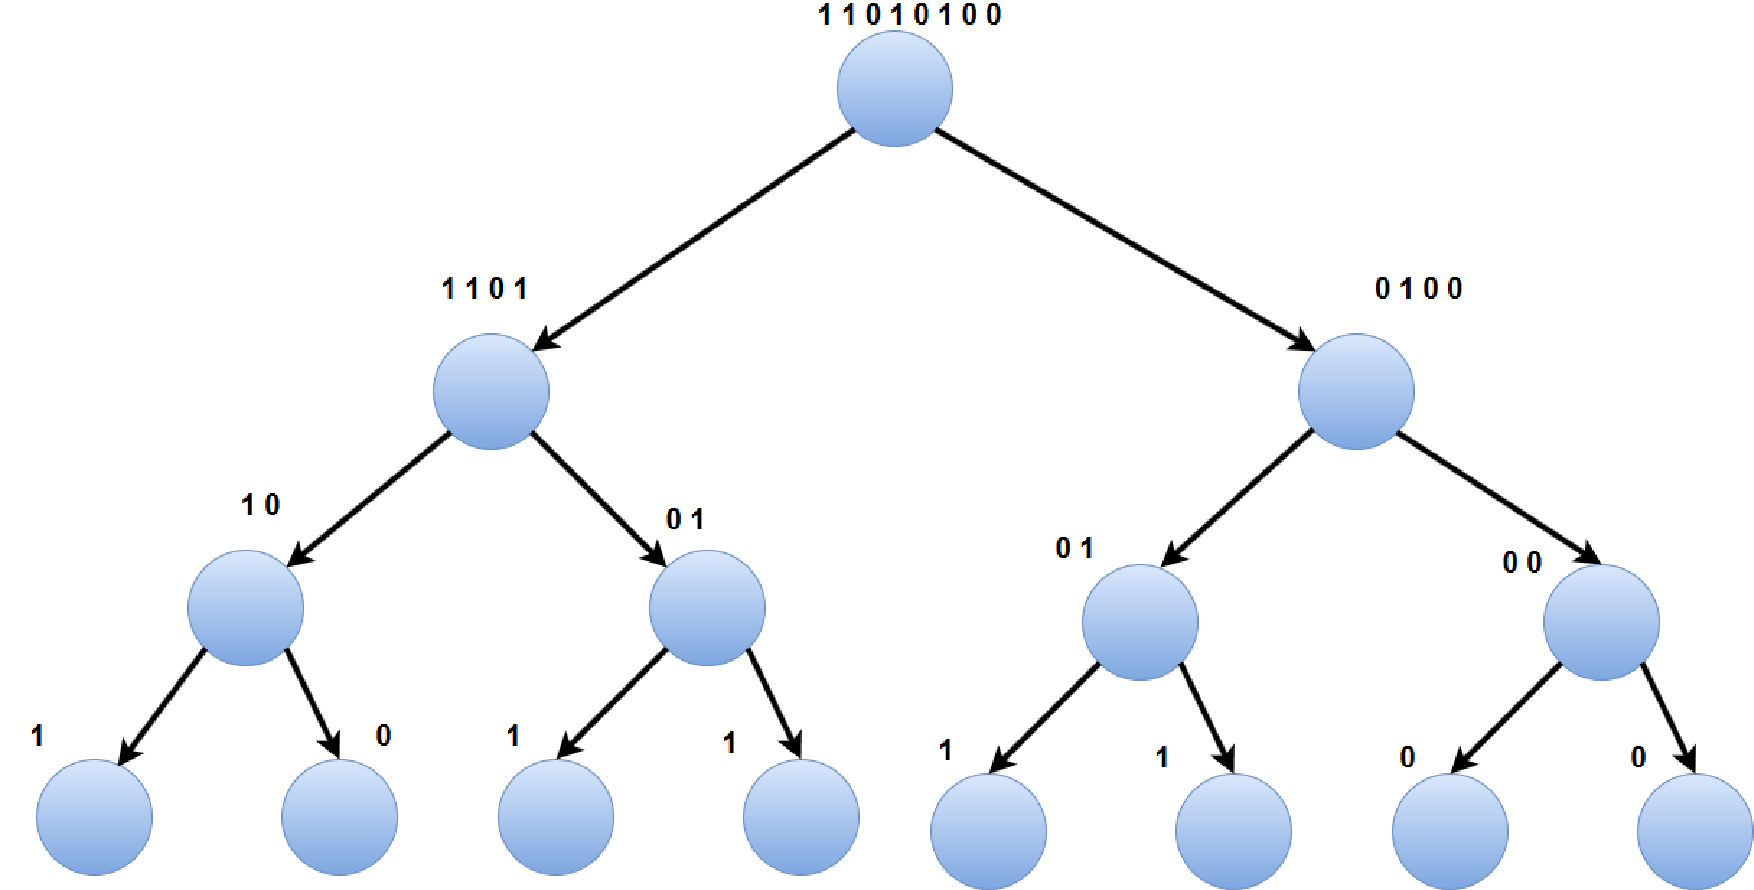
\includegraphics[width=0.7\textwidth]{./figures/treeEncoding.pdf}
	\caption{Encoding tree}
	\label{fig:treeEncoding}
\end{figure}

As it can be observed from the tree, same operation is performed at every node only the size of a vector is different, due to the regular structure encoding problem fits the recursive algorithmic form. Algorithm in ~\ref{algo:polarEncoder} shows a naive implementation of recursive encoder. In the algorithm shown in ~\ref{algo:polarEncoder} each bit is represented a one integer, hence each bit is processed serially parallelism is not exploited. Upon profiling the implementation it also identified that ~\ref{line:copying1} and ~\ref{line:copying2} are also the bottlenecks since copying is involved. One more issue with the algorithm in ~\ref{algo:polarEncoder} is the recursive implementation. Although the encoding can be easily implemented with this algorithm, each recursive function call in software is expensive, since it requires a new stack frame to be allocated each time.

\IncMargin{1.5em}
\begin{algorithm}[]
	\KwData{$u_{\textit{0}}^{\textit{N-1}}$,$N$,$dIndex = 0$}
	\KwResult{$y_{\textit{0}}^{\textit{N-1}}$}
	\SetKwFunction{FMain}{recursiveEncode}
	\SetKwProg{Fn}{function}{:}{}
	\Fn{\FMain{$u_{\textit{0}}^{\textit{l-1}}$,$l$}}{
		\If {$l == 1$} {
			$y_{dIndex} = u_{0}$ \;
			$dIndex = dIndex + 1$ \;
		} \Else {
			$len = \frac{l}{2}$ \;
			$P_{\textit{0}}^{\textit{len-1}}$ = $u_{\textit{0}}^{\textit{len-1}}$ \; 	\label{line:copying1}
			$Q_{\textit{0}}^{\textit{len-1}} = u_{\textit{len}}^{\textit{l-1}}$ \;		\label{line:copying2}
			
			\For{$i=0$ to $length-1$} {													\label{line:xor1}
				$P_{\textit{i}} = P_{\textit{i}} \oplus Q_{\textit{i}}$\;				\label{line:xor2}
			}
			
			\FMain{$P_{\textit{0}}^{\textit{len-1}}$,$len$} \;
			\FMain{$Q_{\textit{0}}^{\textit{len-1}}$,$len$}	\;
		}
	}
	\caption{Naive polar encoder}
	\label{algo:polarEncoder}	
\end{algorithm}
\DecMargin{1.5em}

To avoid the disadvantages mentioned above, following optimization techniques are considered.

$\bullet$ \textbf{Parallel processing:} To avoid the serial processing of bits and for improving the parallelism factor, method described in section ~\ref{dataPackUnpack} is used, i.e is multiple bits are packed to single integer, in this particular instance, every 64 bits of are packed into 64-bit integers so that 64-bits can be processed in parallel with 64-bit supported processor, which results in a parallelism factor ($\mathcal{P}$) of 64. Packing also helps to further increase the parallelism factor $\mathcal{P}$ with state of the art SIMD processing units of the modern processors. SIMD instructions can process of 256-bit or 128-bit in a single instruction which results in a parallelism factor ($\mathcal{P}$) of 256 with AVX and 128 with SSE instructions. \newline
\newline
$\bullet$ \textbf{Avoiding the copy operations:} Naive algorithm in ~\ref{algo:polarEncoder} splits the of $N$-bits into two $\frac{N}{2}$-bit vectors and copies them temporarily allocated variables. Code profiling pointed out that these copying operations are the bottlenecks. In optimized algorithm, instead of copying, C++ pointers concept is used to calculate the index where next block of vector starts and this index is passed to next node for further processing. \newline
\newline
$\bullet$ \textbf{Unrolling the encoder:} Recursive implementation has significant overhead due to the huge number of recursive function calls which require new stack frame allocation. To avoid this overhead, encoder implementation is unrolled, in other words, new inline functions are defined for each vector size. Advantages of these functions is that they don't won't require new stack frame to be allocated when an inline function is called, they will make use of stack frame from which they are called. However this requires a separate inline function for every vector size. Having a different function for every vector size also has advantages, which allows us to use SIMD instructions whenever vector size can fit SIMD registers otherwise normal instructions can be used. \newline
\newline
$\bullet$ \textbf{Pruning encoder tree:} As shown in the figure ~\ref{fig:treeEncoding}, encoding process can be represented as traversal of a binary tree. When an encoding is implemented in software, when traversing the tree towards leaf nodes, bit vector size can becomes less than 8 bits, which requires accessing 4/2/1 bits of an integer. In standard processors smallest unit which can be accessed is an 8-bit integer. To access 4/2/1 bits masking operations are needed. Since the nodes in a binary tree which access 4,2,1 bits is huge, significant number of masking operations are needed, which introduces a added overhead. Pruning of tree at level where the bit vector size is 8, avoids this overhead in addition to reducing the number of nodes to be traversed in a binary tree. Pruning is done by building a lookup table containing encoded value for every combination of 8-bit vector and reading the value from lookup table for the encoded value when the bit vector size is 8. Lookup table will contain 256 bytes, containing encoded value for every combination of 8-bit vector.\newline
\newline
Pruning of the tree had a significant latency improvement, it can be better understood by taking an example. In a scenario where $N = 1024$, with unpruned tree number of nodes to be traversed for encoding is 2047 nodes, out of these nodes contain 1024 1-bit, 512 2-bit and 256 4-bit nodes. With pruned tree 4/2/1 bit nodes are not present, number of nodes to be traversed reduces to 255 from 2047. Pruning avoids masking operations as well as tree traversal. \newline
\newline
Example of a pruned unrolled encoder containing also the tree traversal is shown in the figure ~\ref{fig:unrolledEncoder}. Inline function names for different bit vector size are also shown in the figure. One can see that tree traversing ends at $bitMult8$ function due to pruning. Tree traversal flow is represented with orange line in a figure.

Sample code snippet of node operation with SIMD instructions is shown in a listing.

\begin{figure}[!h]
	\centering
	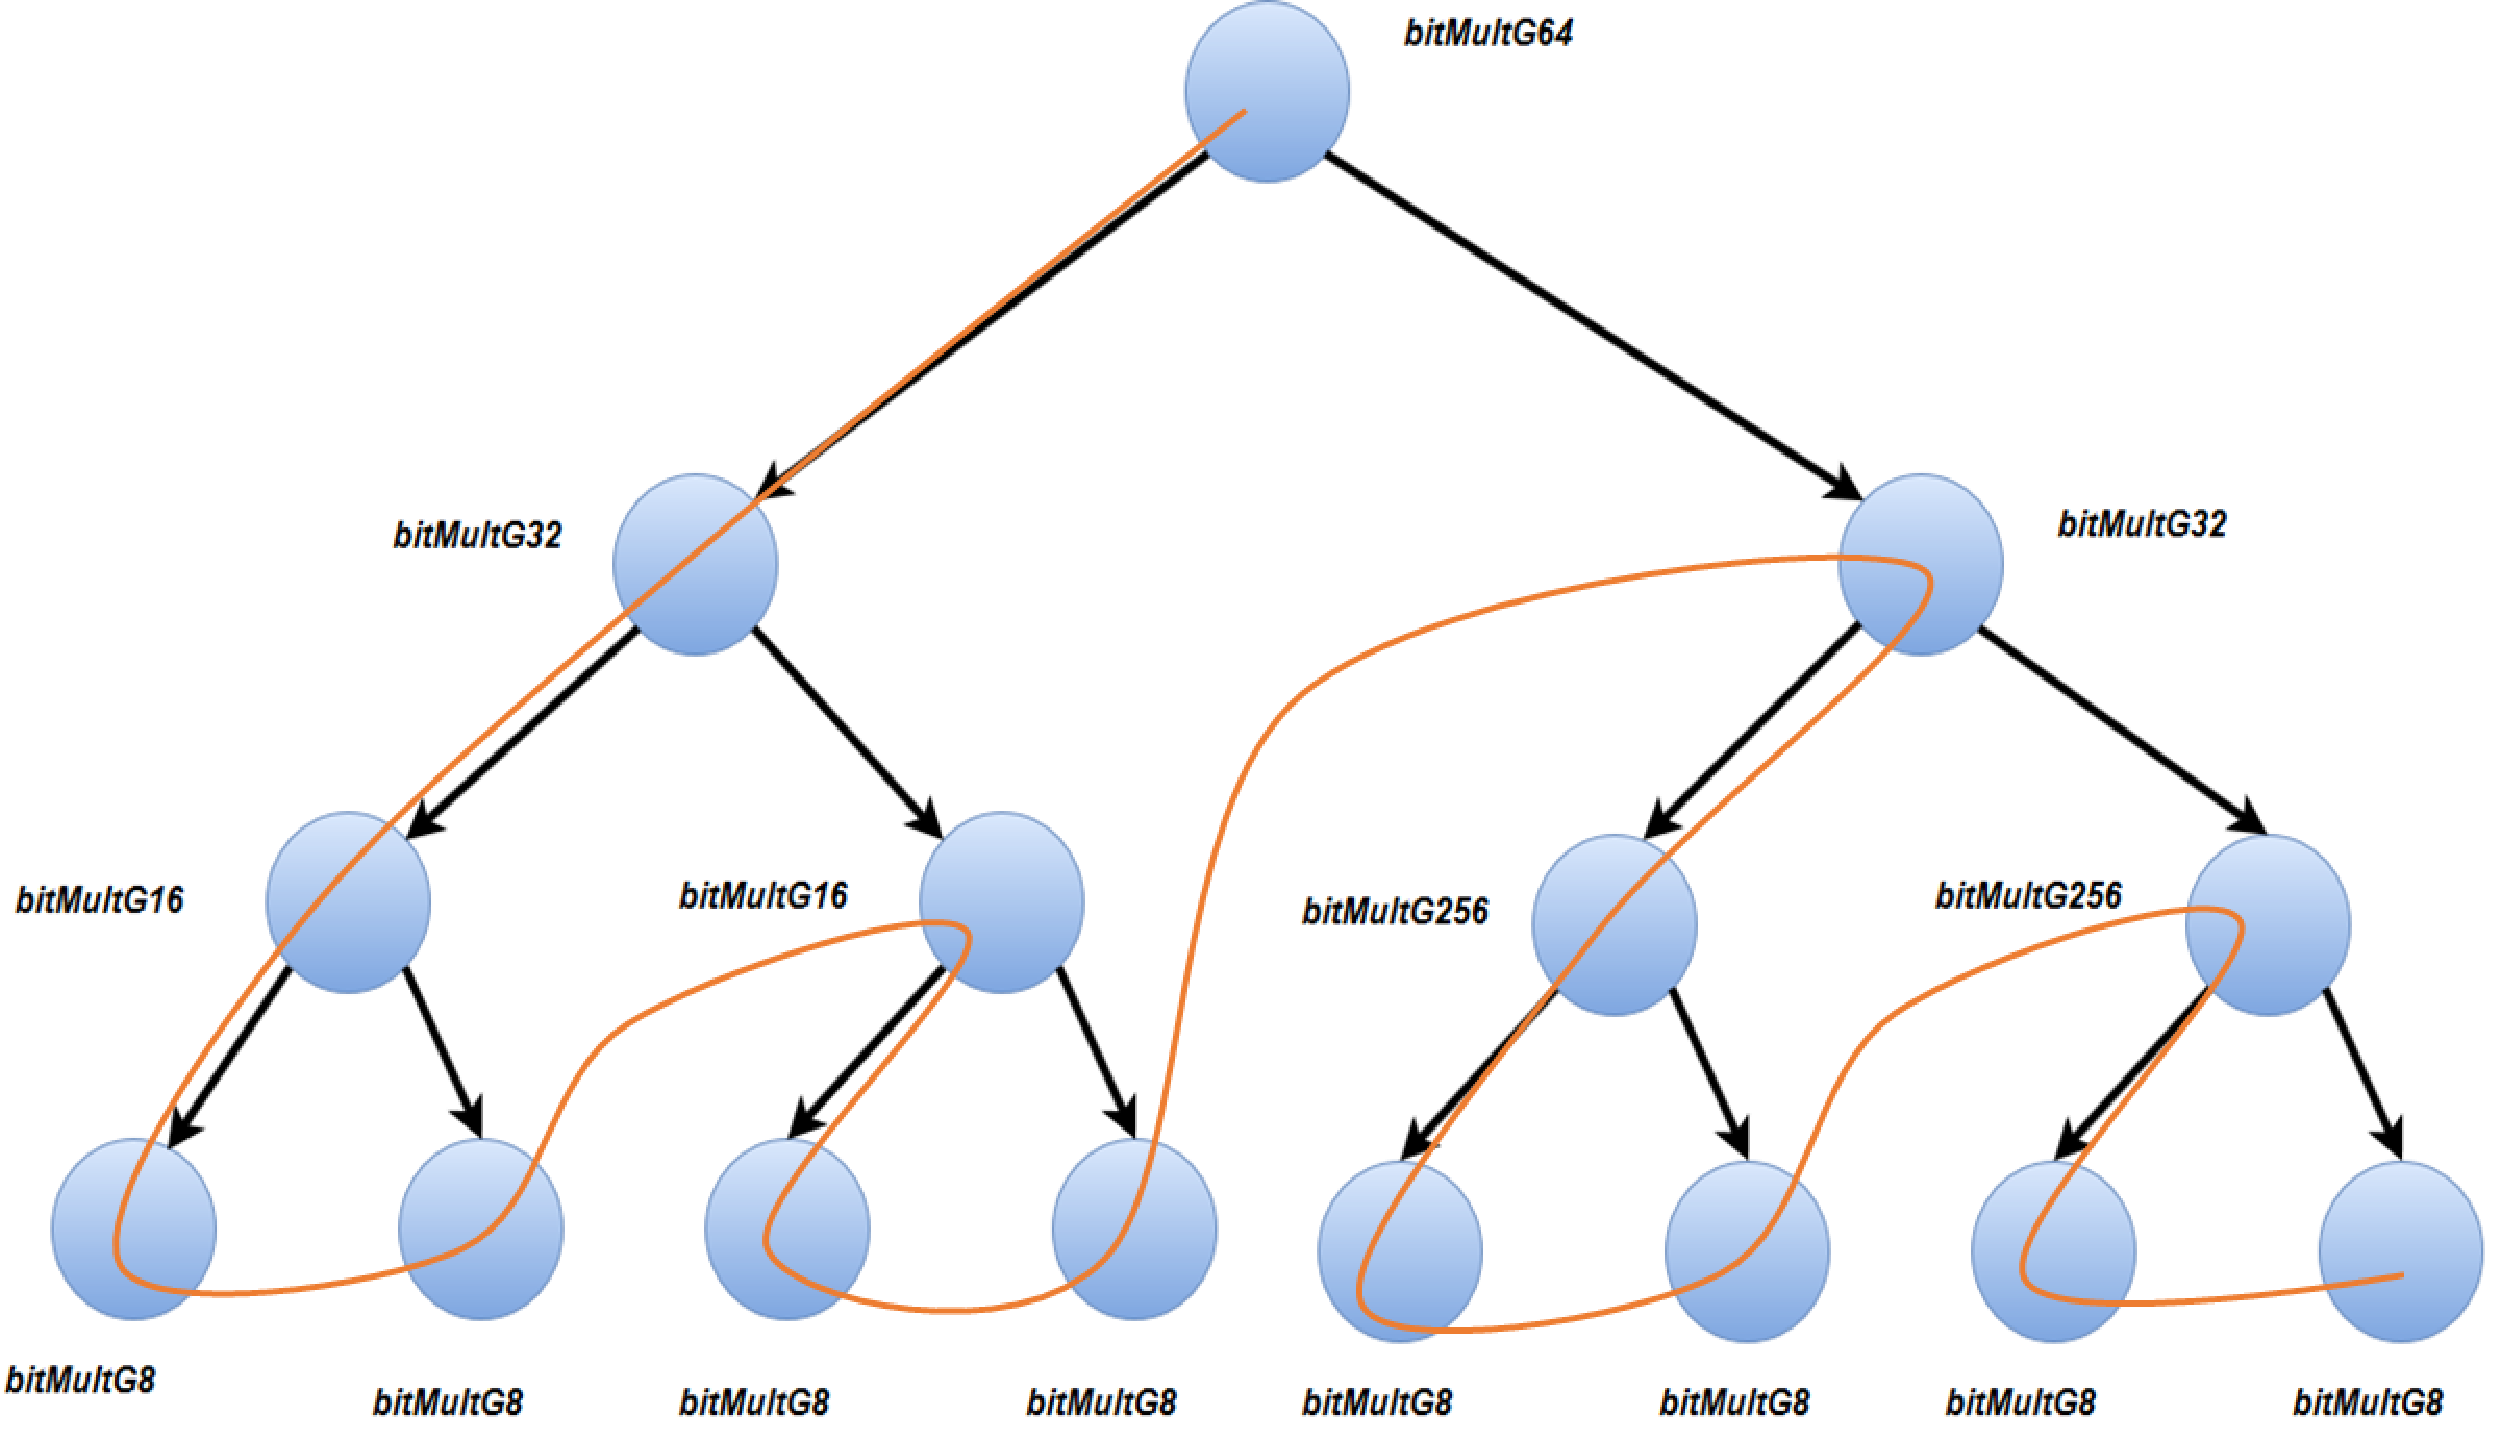
\includegraphics[width=0.7\textwidth]{./figures/unrolledEncoder.pdf}
	\caption{Pruned unrolled encoder tree}
	\label{fig:unrolledEncoder}
\end{figure}

%\TODO{Convert this code to minted format}
\begin{minted}{c}
inline void bitMultG512(uint8_t *s, uint8_t *dEncoded) 
{
	//Here s is 64 bytes, Divided to 32 bytes each.
	uint8_t *s1 = (uint8_t *) s;
	uint8_t *s2 = (uint8_t *) (s + 32);
	__m256i result;
	__m256i temp1 = _mm256_loadu_si256((__m256i*)operand1);
	__m256i temp2 = _mm256_loadu_si256((__m256i*)operand2);
	result = _mm256_xor_si256(temp1,temp2);
	_mm256_storeu_si256((__m256i*)destn, result);
	bitMultG256((uint8_t *) s1, dEncoded);
	bitMultG256((uint8_t *) s2, dEncoded);
}
\end{minted}

\begin{table}[!h]
	\begin{center}
		\caption{Latency comparison: polar encoding for 1024 bits}
		\label{tab:polarEncoder}
		\begin{tabular}{c|c|c} % <-- Alignments: 1st column left, 2nd middle and 3rd right, with vertical lines in between
			\textbf{ } & Naive & Optimized \\
			\hline
			Latency ($\mu$s) & $34$ & $0.244$\\
		\end{tabular}
	\end{center}
\end{table}

\section{Rate matching}
\TODO{Nothing significant for now, Only minor optimizations, May be subblock interleaver can be optimized to reduce the latency by 10us in rate matching process}

\section{Miscellaneous Optimization}
Avoiding multiplication/division and modulus operations and achieving the same using bitwise operations.
Implemented approximate versions $log_{2}x$ and exponential functions to reduce the number of floating point multiplications.
Avoided jump functions to avoid flushing of the instruction pipeline.
Using the compiler optimization primitives to reduce the branches in the program.

\section{Results Comparison}

\subsubsection{PDCCH FEC chain}
Parameters of the FEC chain are n\_max = 9, I\_IL = 1, n\_pc = 0, n\_pc\_wm = 0, I\_BIL = 0, L = 24, E = 423, K = 106.
This is not the worst case, These are the values for parameters specified above.
\begin{table}[!h]
	\begin{center}
		\caption{Latency comparison: PDCCH FEC chain}
		\label{tab:pdcchFecChain}
		\begin{tabular}{c|c|c} % <-- Alignments: 1st column left, 2nd middle and 3rd right, with vertical lines in between
			\textbf{ } & Functional & Optimized \\
			\hline
			Latency ($\mu$s) & $162$ & $19$\\
		\end{tabular}
	\end{center}
\end{table}

\NOTE{PBCH with google benchmark naive = 104us, Optimized = 7.2us, Google benchmark gives reliable reproducible numbers}

\subsubsection{PBCH FEC chain}
Parameters of the FEC chain are n\_max = 9, I\_IL = 1, n\_pc = 0, n\_pc\_wm = 0, I\_BIL = 0, L = 24, E = 864, K = 32.
This is not the worst case, These are the values for parameters specified above.
\begin{table}[!h]
	\begin{center}
		\caption{Latency comparison: PDCCH FEC chain}
		\label{tab:pbchFecChain}
		\begin{tabular}{c|c|c} % <-- Alignments: 1st column left, 2nd middle and 3rd right, with vertical lines in between
			\textbf{ } & Functional & Optimized \\
			\hline
			Latency ($\mu$s) & $53$ & $7$\\
		\end{tabular}
	\end{center}
\end{table}

\NOTE{PBCH with google benchmark naive = 30us, Optimized = 2.3us, Google benchmark gives reliable reproducible numbers}

Worst case latency was for the parameters, 
I\_IL = 1, n\_max = 10, n\_pc = 0 ,n\_pc\_wm = 0, I\_BIL = 1, E = 846, K = 106
Naive 451us, Optimized 40us.